\subsection{Overall accuracy of Simplified Ikeda method}
\label{se:overall_comparison}
An investigation of how well the implementation of the simplified Ikeda's method (see section \ref{se:semi-empirical methods}) agree with the corresponding result in the roll damping database has been carried out. 

Comparing roll damping is a bit difficult since the roll damping model consist of two coefficients, a linear term $B_1$ and a quadratic term $B_2$. These coefficients can be combined by calculating the equivalent linear damping coefficient for a certain roll angle $\phi_a$ \parencite{himeno_prediction_1981}:
\begin{equation}
B_{e} = B_{1} + \frac{8 B_{2} \omega_{0} \phi_{a}}{3 \pi}
\end{equation}


$\phi_a$ was initially taken as the maximum roll angle from the roll decay tests. It was however found that a smaller value of 2 degrees gave better agreement and was instead used.

For the roll damping database $B_1$ and $B_2$ can be inserted directly into equation  \ref{eq:B_e_equation}. 
In order to obtain the same coefficients for the simplified Ikeda's method, roll damping was calculated for two or more roll amplitudes $\phi_a$ for the same motion frequency. $B_1$ and $B_2$ are obtained by fitting equation \ref{eq:B_e_equation} to this data. The $B_e$ coefficient was made non-dimensional according to \parencite{himeno_prediction_1981} giving the non-dimensional equivalent linear damping coefficient $\hat{B_e}$, which was more convenient to use for this comparison. 

It was found that almost all ships in the roll damping database were outside the limits in equation \ref{eq:SI_limits}). Two different ways to handle this limit exceedance was investigated: one "unlimited" approach where the input values where allowed to exceed the limits and one "limited" approach where the limit boundary values were used for exceeding values. Figure \ref{fig:ikeda_limited} show predictions with the Simplified Ikeda's method using the "unlimited" and "limited" approach compare to the corresponding results from model tests. The "limited" approach seems to be the best one to use according to this figure, where the "unlimited" approach has values very far away from the red reference line.   

\begin{figure}[H]
\centering
  \centering
  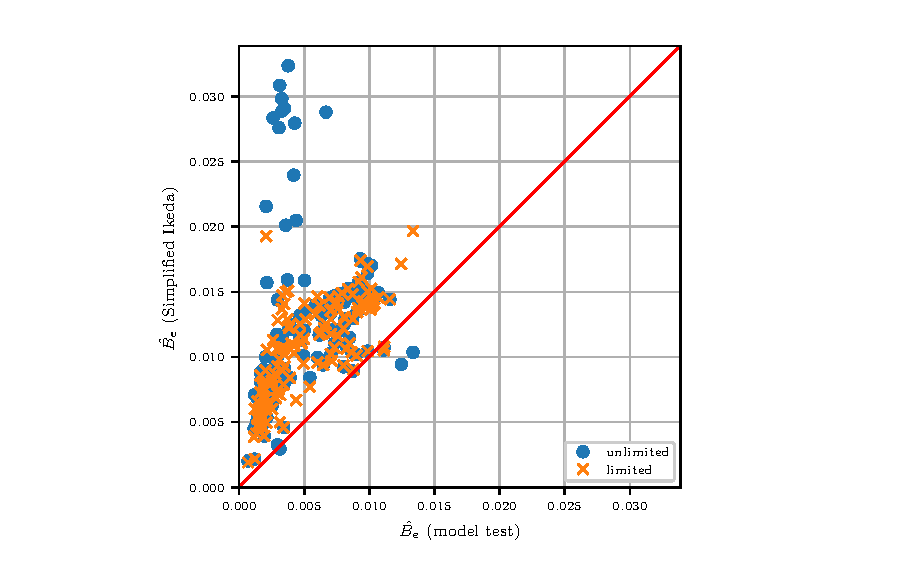
\includegraphics[height=8cm]{figures/ikeda_limited.eps}
  \caption{$\hat{B_e}$ comparison at all speeds}
  \label{fig:ikeda_limited}
\end{figure}



\begin{figure}[H]
\centering
  \centering
  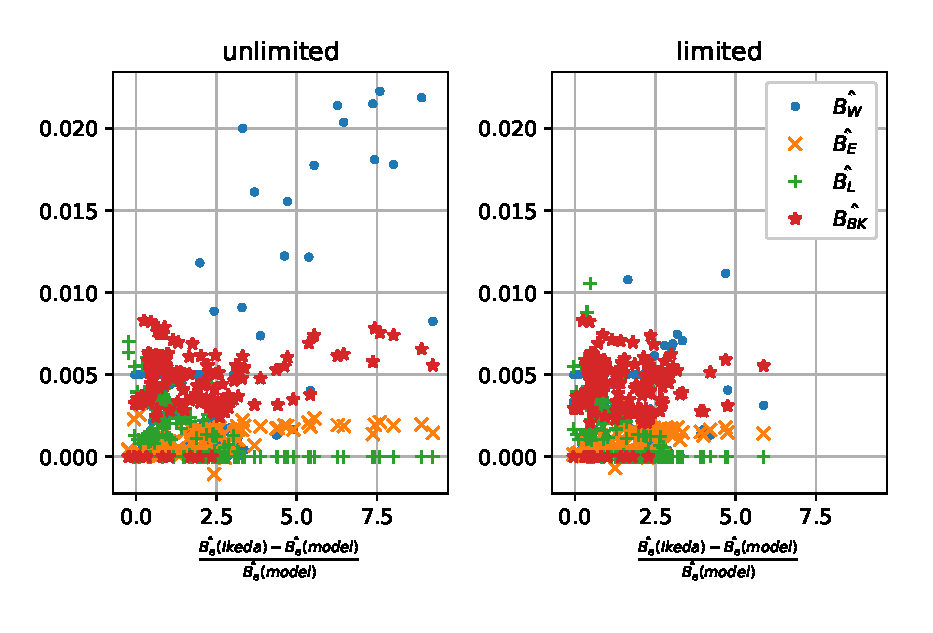
\includegraphics[height=8cm]{figures/ikeda_components.eps}
  \caption{Deviation versus simplified Ikeda roll damping components}
  \label{fig:ikeda_limited}
\end{figure}



\textcolor{red}{\subsection{Improved S1 in literature?}}
The eddy damping $ B_E $ becomes negative when $ C_b>0.84 $ according to \parencite[]{rudakovic_application_2017}.

